%%%%%%%%%%%%%%%%%%%%%%%%%%%%%%%%%%%%%%%%%%%%%%%%%%%%%%%%%%%%%%%%%%%%%%%
%                          template.tex
%
% LaTeX template for papers conforming to the United States Sections of
% the Combustion Institute style guide.
%
% Authors:
%     Bryan W. Weber, University of Connecticut
%     Kyle E. Niemeyer, Oregon State University
%
% This work is licensed under the Creative Commons Attribution 4.0
% International License. To view a copy of this license, visit
% http://creativecommons.org/licenses/by/4.0/.
%%%%%%%%%%%%%%%%%%%%%%%%%%%%%%%%%%%%%%%%%%%%%%%%%%%%%%%%%%%%%%%%%%%%%%%

\documentclass[12pt]{ussci}

%======================================================================
% packages
\usepackage{textgreek}
\usepackage{amsmath,amsfonts,amssymb}
\usepackage{graphicx}
\usepackage{float}
\restylefloat{table}
\usepackage{booktabs} % for much better looking tables
\usepackage{array} % for better arrays (eg matrices) in maths
\usepackage{paralist} % very flexible & customisable lists (eg. enumerate/itemize, etc.)
\usepackage{listings}
\usepackage{verbatim} % adds environment for commenting out blocks of text & for better verbatim
\usepackage{caption}
\usepackage{subcaption} % make it possible to include more than one captioned figure/table in a single float
\usepackage{multirow}
\usepackage{rotating}
\usepackage{ulem}
\usepackage{bigstrut}
\usepackage{bm}
\usepackage[space]{grffile}
\usepackage{tikz}
\usetikzlibrary{shapes.geometric, arrows}
\usetikzlibrary{calc,patterns,angles,quotes,shapes,positioning}
\usepackage{xspace}
\usepackage{enumitem}
\usepackage[version=4]{mhchem}

%better printing of numbers
\usepackage[T1]{fontenc}
\usepackage[english]{babel}
\usepackage{csquotes}
\usepackage{textcomp}

\usepackage{siunitx}
\sisetup{group-separator={,},
     detect-all,
     binary-units,
     list-units = single,
     range-units = single,
     tophrase = --,
     per-mode = symbol-or-fraction,
     separate-uncertainty = true,
     list-final-separator = {, and }
%    scientific-notation = fixed
}
\DeclareSIUnit\atm{atm}

\newcommand{\degree}{\ensuremath{{}^{\circ}}\xspace}
\usepackage{listings}
\usepackage{blindtext}
\usepackage{subfiles}
\usepackage{breakcites}
%======================================================================
% Add your bibliography file here, replace template.bib
\addbibresource{mendeley.bib}
%======================================================================
% Replace "Reaction Kinetics" in the line below by your paper topic
\newcommand\papertopic{Reaction Kinetics}
%======================================================================

\graphicspath{{./Figures/}}

\title{ Investigating stiffness detection metrics for chemical kinetics }

\author[1]{Andrew Alferman}
\author[1,*]{Kyle E. Niemeyer}


\affil[1]{School of Mechanical, Industrial, and Manufacturing Engineering\\
		Oregon State University, Corvallis, OR 97331, USA}
\affil[*]{Corresponding author: \email{Kyle.Niemeyer@oregonstate.edu}}


\begin{document}
\maketitle

%====================================================================
\begin{abstract} % not to exceed 200 words

%Abstract should be between 150--200 words and should state briefly the purpose of the research, the principal results and major conclusions. An abstract is often presented separately from the article, so it must be able to stand alone. For this reason, References should be avoided, but if essential, then cite the author(s) and year(s). Also, non-standard or uncommon abbreviations should be avoided, but if essential they must be defined at their first mention in the abstract itself.

Simulations of combustion and reacting flows often encounter stiffness in the equations governing chemical kinetics.
Explicit solvers for these ordinary differential equations offer low computational expense, but typically cannot efficiently handle stiff systems.
In contrast, implicit methods demand greater expense but offer unconditional stability\textendash as a result, most reactive flow solvers rely on these methods by default (other than explicit direct numerical simulation solvers).
However, explicit or stabilized explicit methods can instead be used to reduce the computational expense while remaining stable and accurate if the chemical kinetics systems exhibit low-to-moderate stiffness.
This study investigates metrics for quantifying stiffness, with the goal of identifying one capable of efficiently and robustly determining the appropriate category of integrator required.
Methods of measuring the stiffness of chemical kinetics states will be investigated, including stiffness ratio, stiffness index, stiffness indicator, and chemical explosive mode.
These will be applied to simulations of hydrogen/carbon monoxide and methane autoignition using initial conditions representative of realistic turbulent combustion, obtained from partially stirred reactor simulations.
The stiffness quantification metrics will be compared with the time required to integrate using implicit and explicit methods.
We will conclude by analyzing preliminary performance analysis of an integrator scheduler using these metrics.

\end{abstract}

% Provide 2-4 keywords describing your research. Only abbreviations firmly
% established in the field may be used. These keywords will be used for
% sessioning/indexing purposes. Use \sep between each keyword.
\begin{keyword}
    Stiffness quantification\sep Ordinary differential equations\sep Chemical kinetics\sep Computational cost reduction
\end{keyword}

%====================================================================
\section{Introduction}
%

An increasing demand for greater efficiency and lower \ce{CO2} emissions in the US energy supply has driven the development of next-generation combustion technologies that use alternative fuels \cite{Epstein2012}.
Computational modeling is one important tool that increasingly drives design and development of these new technologies.
Shortening the design cycle and time-to-market of novel and efficient energy devices optimized for alternative fuels requires fundamental advances in combustion science and fuel chemistry; both depend on high-fidelity computational tools~\cite{Niemeyer}.
The need to develop new, high-performance computational methods to support combustion research has been recognized by multiple federal agencies as a key objective towards implementing predictive models~\cite{Trouve:2006tq,DOE:2007tj,NationalResearchCouncil:2011ub,National-Research-Council:2014aa}.

Species time scales can range from the order of nanoseconds to seconds, requiring greater computational expense for integration by conventional methods (i.e., numerical stiffness)~\cite{Lu2009}.
Most combustion modeling approaches rely on a single, implicit ODE integration method to handle the chemistry in all spatial locations, but these methods are computationally expensive, especially for larger mechanisms.
The computational cost of chemistry is either a quadratic or cubic function of the number of species~\cite{Lu2009}; reaction mechanisms of sizes comparable to those shown above pose computational difficulties even in zero-dimensional (homogeneous) simulations.

Depending on the local conditions, computational flow time-step size, and chemical mechanism being used, it is possible to encounter a wide range of stiffness within a single simulation.
We can exploit this situation to reduce the overall simulation expense by selecting the most computationally efficient ODE solver on-the-fly based on local conditions.
For example, a low-cost explicit method may be used far away from the reaction zone, while an implicit---or otherwise ``stiff''---solver is more economical inside a flame.
Making this selection requires a method to detect and classify stiffness~\cite{Niemeyer}.

Although the concept of stiffness has been identified for over 60 years, the term has not been precisely defined despite repeated efforts.
The diverse set of problems considered to be ``stiff'' and the large variety of characterizations used to describe stiffness are amongst the difficulties that have been encountered in developing a precise definition~\cite{Soderlind2014}.
Nonetheless, a variety of stiffness quantification methods have been developed with the goal of providing a practical means of evaluating a systems ODEs~\cite{Soderlind2014,Shampine1985,Brugnano2011,Lambert1973ComputationalEquations,Hairer1996SolvingII}.
We look to these methods of stiffness quantification to determine their usefulness with respect to the equations governing combustion, and to determine if a reliable and efficient means of switching methods can be developed from it.
In doing so, we hope to reduce the computational expense of combustion simulations.

\section{Methods}
We considered two different chemical kinetic models in this study: the relatively small hydrogen\slash carbon monoxide (\ce{H2}\slash \ce{CO}) model of Burke et al.~\cite{Burke:2011fh} and GRI Mech 3.0~\cite{grimech3}, which uses \ce{CH4} as fuel.
The \ce{H2}\slash \ce{CO} model uses 13 species while the GRI Mech 3.0 is larger and uses 53 species, allowing for Jacobian matrices of system of ODEs of $13 \times 13$ and $53 \times 53$, respectively.
These relatively small Jacobian matrices allow for much faster evaluations of stiffness than would be possible with larger, more complicated kinetic systems, which can have hundreds to hundreds of thousands of chemical species~\cite{Niemeyer:2013}.

The code used to run autoignition simulations and calculate stiffness metrics was written in Python and made use of open-source software, including the \texttt{ode} integrator function of SciPy~\cite{SciPy}.
Two different integrators of the \texttt{ode} integrator function were used to compare explicit to implicit methods. 
The first integrator was \texttt{vode}, which uses an implicit Adams method for non-stiff problems and a method based on the backwards differentiation formulae (BDF) for stiff problems~\cite{Brown1989}.
The explicit integrator used was \texttt{dopri5}, which uses a Runge-Kutta method of order (4)5 developed by Dormand and Prince with automatic step size control~\cite{E.HairerSPNorsett1990}.
The \texttt{vode} integrator was set to use the default behavior of using first-order finite differencing to provide an estimate of the Jacobian matrix.
Both integrators use internal time-steps in between the user defined time-steps for accuracy control and make use of \texttt{FORTRAN} libraries to perform the integrations.
\texttt{NumPy}~\cite{VanDerWalt2011} was also extensively used in the code to determine eigenvalues and perform numerous basic mathematical functions.
The integrator used default values of \num{e-6} and \num{e-12} for the error control parameters \texttt{rtol} and \texttt{atol}, respectively.

Computation of the right hand side (RHS) function and the Jacobian matrix of the systems of ODEs were readily achieved using pyJac~\cite{pyJac:1.0.2}, a Python-based open-source program that generates analytical Jacobian matrices for use in chemical kinetics modeling and analysis~\cite{Niemeyer:2017}.
pyJac uses a chemical mechanism developed using Cantera~\cite{Goodwin:2015aa} software and a set of initial conditions to generate functions that return the required values.

Our analysis was conducted using information gathered from partially stirred reactor (PaSR) simulations.
As described by Niemeyer et al.~\cite{Niemeyer:2017}, the PaSR model consists of a number of particles, each with a time-varying composition.
At discrete time-steps, events including inflow, outflow, and pairing cause particles to change composition; between these time-steps, mixing and reaction fractional steps evolve the composition of all particles.
By using data from a single particle of the PaSR model, the evaluation could be simplified to a zero-dimensional analysis.
The \ce{H2}\slash \ce{CO} simulation used a different set of PaSR data than the GRI Mech 3.0 simulation.
Both sets of PaSR data included nine different configurations of temperature and pressure; the initial temperature values were 400, 600, and 800 K, while the pressure values were 1, 10, and 25 atm.
Pressure remained constant throughout the simulations.

The wall clock time required by \texttt{vode} and \texttt{dopri5} to advance one user specified time step was measured for each particle of the PaSR simulation.
The number of RHS function calls used by the integrator to advance one time-step was measured by adding a global variable, and the number of internal time-steps used by \texttt{vode} was measured.
Measurement of the time-steps used by \texttt{vode} was accomplished without manipulation of the original \texttt{FORTRAN} code by limiting the integrator to one time step each time the integrator was called.
\texttt{dopri5} is explicit and uses six function calls to advance each internal time step, therefore the number of internal time-steps for this integrator was calculated by dividing the number of RHS function calls by six.

% Not sure why this one was here in the last paper.
% (Please refer to Niemeyer et al.~\cite{Niemeyer:2017} for a detailed description of the relevant equations and solution technique.)

The four stiffness quantification methods discussed within this paper are the stiffness ratio, the stiffness index, the stiffness indicator, and the chemical explosive mode.
Variable names have been changed in the equations below to maintain consistency throughout this paper.

\subsection{Stiffness Ratio}
One commonly referenced measure of the stiffness of a system of ODEs is the ``stiffness ratio.''
The stiffness ratio of the system of ODEs is defined as
\begin{equation}
	\textrm{Stiffness Ratio} = \frac{\textrm{max}|\lambda_p|}{\textrm{min}|\lambda_p|}
\end{equation}
in which $\lambda_p$ is an eigenvalue of the Jacobian matrix of the system of ODEs~\cite{LeVeque2007}.
A large stiffness ratio is an indication of a large range of time scales in the problem, which is a necessary component for stiffness to arise.
This method is readily implemented and carries little computational cost beyond determining the eigenvalues of the Jacobian matrix.

\subsection{Stiffness Index}

One method of interest regarding stiffness quantification was the ``IA-Stiffness Index'' proposed by Shampine~\cite{Shampine1982}.
This method enables comparison of values of the stiffness index between different equations and different methods.
Additionally, the method takes into account the impact of the order of the method selected when evaluating the stiffness.
The method is relatively straightforward to implement, requiring computation of a vector of the derivatives of the system of equations, as well as either a weighted norm or the spectral radius of the Jacobian matrix.

% Replaced the Jacobian $f_y(x_n,y(x_n))$ with $A$ to keep consistent nomenclature
The IA-stiffness index of a method of order \textit{p} introduced by Shampine~\cite{Shampine1982} is
\begin{equation}
    \frac{h_{acc}}{h_{iter}} \doteq \tau ^ {1/(p + 1)} \rho [A] \|y^{(p+1)}(x_n)\|^{-1/(p+1)} \left( \frac{|\xi|^{-1/(p+1)}}{|\gamma|} \right)
\end{equation}
or alternatively,
\begin{equation}
    \frac{h_{acc}}{h_{iter}} \doteq \tau ^ {1/(p + 1)} \|A\|\|y^{(p+1)}(x_n)\|^{-1/(p+1)} \left( \frac{|\xi|^{-1/(p+1)}}{|\gamma|} \right)
\end{equation}
where $h_{acc}$ represents the largest step size which would result in a local accuracy test being passed, $h_{iter}$ represents the minimum step size that will lead to divergence of simple iteration, $\tau$ represents the specified tolerance, $\rho [A]$ represents the spectral radius of the Jacobian matrix $A$, $\gamma$ is a constant characteristic of the formula, and $\xi$ represents a constant characterizing the accuracy of a reference method.
Note that these equations require the $p+1$ derivative of the function $y(x_n)$.
Additionally, the matrix norm $\|M\|$ of matrix $M$ with $i$ columns and $j$ rows is given by
\begin{equation}
    \|M\| = \max_{i} \frac{1}{w_i} \sum_{j} |M_{ij}|w_j
\end{equation}
in which \(w_i\) and \(w_j\) are positive weights of the matrix~\cite{Shampine1985}.

Although the IA-stiffness index is useful in determining the stiffness of a method for a given system of equations, we are interested in quantifying the stiffness inherent to the system of equations itself.
Such a quantification is necessary for investigating method switching mechanisms.
Shampine notes that the scalar quantity
\begin{equation}\label{eqn:stiffness}
    \textrm{Stiffness Index} = \rho [A] \|y^{(p+1)}(x_n)\|^{-1/(p+1)}
\end{equation}
provides a fair ``stiffness index'' to a given problem~\cite{Shampine1985}. For the remainder of this document, all references to the stiffness index will refer to the value obtained using equation (\ref{eqn:stiffness}).
A large value of the stiffness index at a given point is an indication that the system of ODEs is locally stiff at that point.

As previously noted, use of the above equations requires calculation of a vector of the derivatives of a system of equations.
In the case of this investigation, this vector is comprised of the derivatives of the thermochemical composition vector with respect to time, with the the vector defined as
\begin{equation}
    \Phi = \{T, Y_1, Y_2, \dots, Y_{N_{sp}} \}^\intercal \;,
\end{equation}
where $T$ is the temperature, $Y_i$ are the species mass fractions, and $N_{sp}$ is the number of species in the mechanism~\cite{Niemeyer:2017}.
The vector needed to compute the stiffness index is therefore
\begin{equation}
    \frac{\partial \Phi}{\partial t} = \left\{\frac{\partial Y_1}{\partial t}, \frac{\partial Y_2}{\partial t}, \dots, \frac{\partial Y_{N_{sp}}}{\partial t} \right\}^\intercal \;,
\end{equation}
where time is denoted by $t$~\cite{Niemeyer:2017}.
In addition to this vector of derivatives, computation of the stiffness index requires either the weighted norm or the spectral radius of the Jacobian matrix for the thermochemical composition vector.

After generating this data using pyJac, the values of the second derivative of the thermochemical composition vector were calculated numerically using a fourth-order central differencing formula.
Numerical approximations of higher-level derivatives may also be generated using the same approach.
Use of the central differencing formula was possible because the stiffness index was calculated after solving for the thermochemical composition vector, and the reaction was modeled using user defined time-steps of a constant size.
Forward and backward difference formulae were used at the boundaries where central differencing could not be used.
Variable time-step methods for calculating the second derivative or higher-level derivatives may also be used, however these methods were not necessary at the current stage of the investigation.

To facilitate comparison of the results obtained by Shampine~\cite{Shampine1985}, the order of the method was assumed to be 1 for all computations performed in this paper.

\subsection{Stiffness Indicator}
The ``stiffness indicator'' of a system of ODEs was proposed by S{\"o}derlind et. al. as a mathematically rigorous approach to characterize stiffness that works independent of the integration method used or operational criteria~\cite{Soderlind2014}.
S{\"o}derlind notes that ``large'' negative values of the stiffness indicator are a necessary condition for stiffness.
S{\"o}derlind further quantifies how ``large'' the negative values must be for an equation to be considered locally stiff for a given problem, however we are primarily interested in the values of the stiffness indicator itself to facilitate comparison between different simulations using different models and different timescales.

In the chemical kinetic models of interest, the stiffness indicator is calculated for a given Jacobian matrix $A \in \mathbb{R}^{n \times n}$ as:
\begin{equation}
	\textrm{Stiffness Indicator} = \frac{m[A] + M[A]}{2}
\end{equation}
where
\begin{equation}
	m[A] = \textrm{min}\,\lambda[\textrm{He}(A)];\qquad M[A] = \textrm{max}\,\lambda[\textrm{He}(A)],
\end{equation}
with $\lambda [A]$ denoting the eigenvalues of matrix $A$ and $\textrm{He}(A)$ denoting the Hermitian part of the matrix $A$, which is defined as
\begin{equation}
	\textrm{He}(A) = \frac{A + A^\intercal}{2}.
\end{equation}
While determination of the stiffness indicator does require calculation of eigenvalues following a transpose and addition of the Jacobian matrix, it is readily implemented and unlike the stiffness index it does not require storage of prior values of the solution.

\subsection{Chemical Explosive Mode}
The ``chemical explosive mode analysis'' (CEMA) was developed as a diagnostic to identify flame and ignition structure in complex flows~\cite{Yoo2009}.
Though this metric was not originally intended as a device to quantify the numerical stiffness of a system of ODEs, we are interested in determining if correlations exist between identification of the flame structure and the computational work required to advance the simulation for either explicit or implicit methods.
The chemical explosive modes are associated with positive eigenvalues of the Jacobian of the system of ODEs:
\begin{equation}
	\textrm{Re}(\lambda) > 0.
\end{equation}
Similar to the stiffness ratio, the CEMA is readily implemented and carries little computational cost beyond determining the eigenvalues of the Jacobian matrix.

\section{Results and Discussion}

An analysis of each stiffness metric was performed using every particle in the PaSR simulation.
In this analysis, a simulation at each particle of the PaSR was advanced only as long as needed to obtain an accurate numerical value of each stiffness metric.
Because a fourth order central difference formula was used to numerically approximate the second derivatives in the calculation of the stiffness index, the simulation was advanced until five solution values existed at each particle.
The only information needed to calculate the stiffness ratio, stiffness indicator, and chemical explosive modes is the Jacobian matrix, therefore these values could be calculated at every time-step as soon as the solution was known.
Constant step sizes of $1 \times 10^{-7}$ s and $1 \times 10^{-8}$ s were used for computations of the \ce{H2}\slash \ce{CO} model and GRI Mech 3.0 models, respectively, however the built in methods of the \texttt{ode} package have automatic step size control to ensure that values remain within tolerance, and the integrator may take many steps in between the specified time-step.
Using state data obtained during the simulation, the Jacobian matrix was calculated at each time-step using \texttt{pyJac}, which allowed the numerical values of each stiffness matrix to be calculated.
As previously discussed, the wall clock time, number of RHS function calls, and internal time-steps were measured once at each particle, however we are most interested in wall clock time for the purposes of this study.
The simulation was performed on an early 2015 MacBook Pro with a 2.9 GHz Intel Core i5 processor.

\subsection{Results}
The \ce{H2}\slash \ce{CO} model was examined first due to its relative simplicity.
The PaSR data for the this model consisted of 900900 different particles.
It was found that \texttt{vode} had a smaller clock time than \texttt{dopri5} for 729384 particles or 81.0\% of the PaSR data for this model, while \texttt{dopri5} had a smaller clock time for 165001 particles or 18.3\% of the PaSR data.
\texttt{vode} and \texttt{dopri5} had the same clock time within the numerical tolerance of the Python code for 6515 particles, and \texttt{dopri5} did not fail when integrating at any particle.
% A depiction of the number of function calls used by both \texttt{vode} and \texttt{dopri5} can be found in Figure~\ref{fig:WCTH2COPaSR}.
In general, \texttt{vode} was likely to outperform \texttt{dopri5} when pressure was 1 atm, and also when pressure was 10 atm at 400K.
At higher pressures and temperatures, the explicit \texttt{dopri5} was more likely to outperform the implicit \texttt{vode} when using this model.
This may be because the \ce{H2}\slash \ce{CO} model is generally more limited by accuracy requirements as opposed to stability requirements.
\texttt{vode} uses backward differentiation formulae, which require multiple data points for higher order approximations.
At the boundary conditions where few or no adjacent data points exist, lower order approximations are used.
The use of lower order methods may be advantageous when few internal time-steps are needed because fewer RHS function calls are required to provide an approximation.
Higher order methods may be advantageous when an intermediate number of time-steps are needed to provide the required accuracy because higher order methods are often able to make use of larger time-steps.
Additionally, unlike implicit methods, explicit methods do not require calculation of Jacobian matrices to advance time.

\begin{figure}[htbp]
    \centering
%    \begin{subfigure}{0.43\textwidth}
%        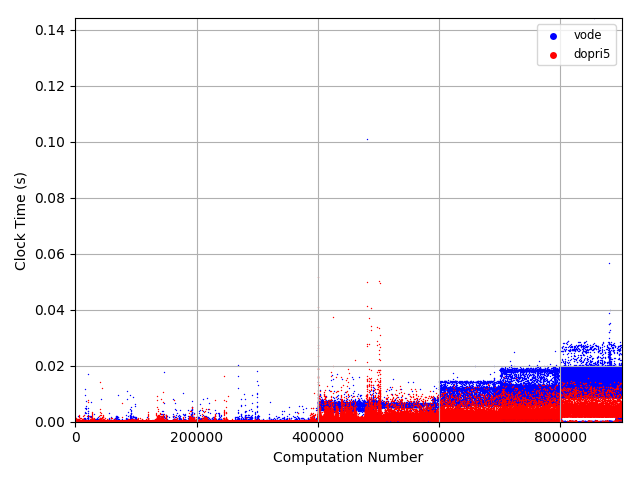
\includegraphics[width=\linewidth]{H2_CO/PaSR_Int_Times_1e-07.png}
%        \caption{Wall clock time required to integrate one time-step for both \texttt{dopri5} and \texttt{vode} at each particle of the PaSR model.}
%        \label{fig:WCTH2COPaSR}
%    \end{subfigure}
    \begin{subfigure}{0.43\textwidth}
        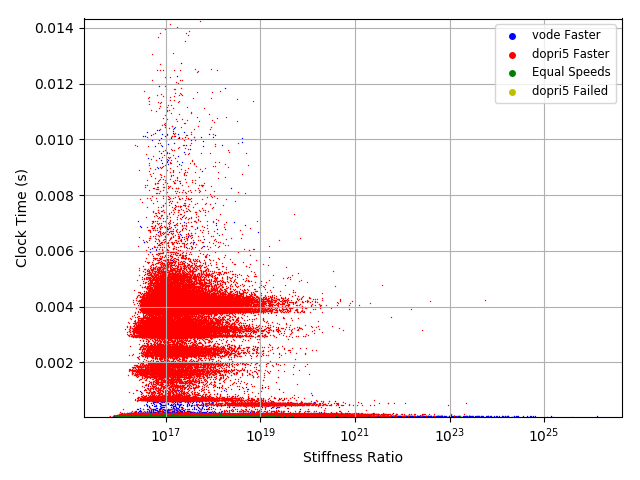
\includegraphics[width=\linewidth]{H2_CO/PaSR_Int_Times_Ratio_Groupings_1e-07.png}
        \caption{Stiffness ratio versus wall clock time used to integrate one time-step at each particle of the PaSR model.}
        \label{fig:SRH2COPaSR}
    \end{subfigure}
    \hfill
    \begin{subfigure}{0.43\textwidth}
        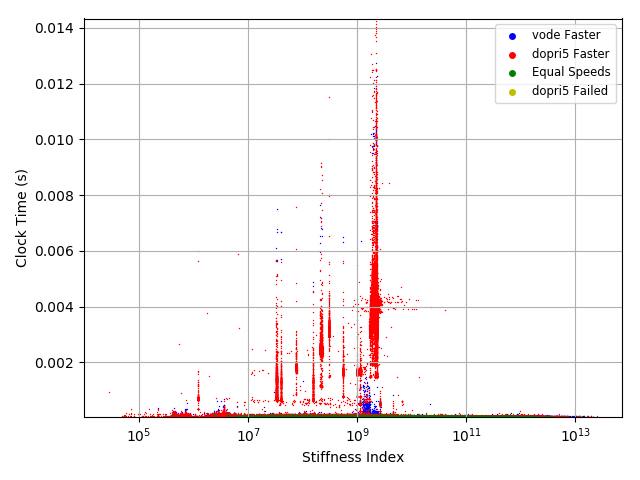
\includegraphics[width=\linewidth]{H2_CO/PaSR_Int_Times_Index_Groupings_1e-07.png}
        \caption{Stiffness index versus wall clock time used to integrate one time-step at each particle of the PaSR model.}
        \label{fig:SI1H2COPaSR}
    \end{subfigure}
    \begin{subfigure}{0.43\textwidth}
        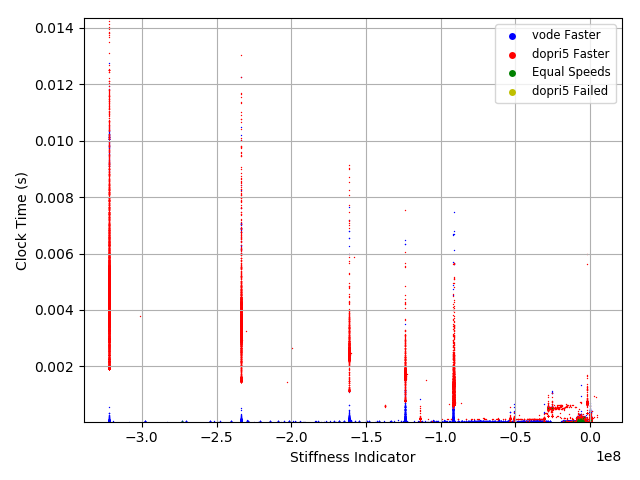
\includegraphics[width=\linewidth]{H2_CO/PaSR_Int_Times_Indicator_Groupings_1e-07.png}
        \caption{Stiffness indicator versus wall clock time used to integrate one time-step at each particle of the PaSR model.}
        \label{fig:SI2H2COPaSR}
    \end{subfigure}
    \hfill
    \begin{subfigure}{0.43\textwidth}
        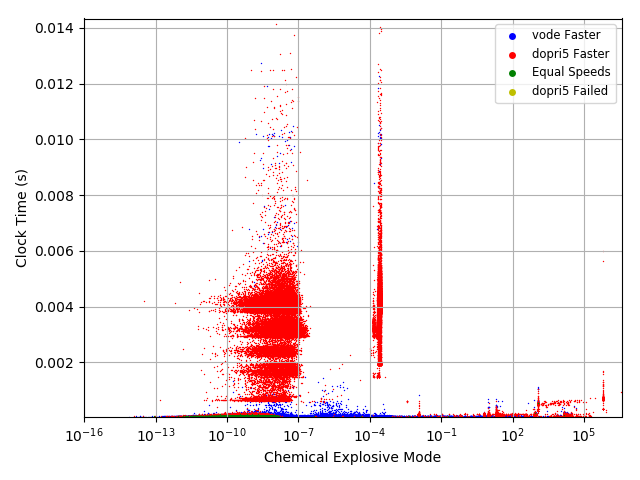
\includegraphics[width=\linewidth]{H2_CO/PaSR_Int_Times_CEMA_Groupings_1e-07.png}
        \caption{Chemical explosive mode versus wall clock time used to integrate one time-step at each particle of the PaSR model.}
        \label{fig:CEMH2COPaSR}
    \end{subfigure}
    \caption{Stiffness metrics versus RHS function calls used to advance one time-step of the \ce{H2}\slash \ce{CO} model using either \texttt{vode} or \texttt{dopri5}.  Calculated with a user defined constant step size of \SI{e-7}{\second} for every initial condition represented in the PaSR model.}
    \label{fig:H2COPaSRStiffness}
\end{figure}

As seen in Figure~\ref{fig:SRH2COPaSR}, the stiffness ratio was not highly correlated with wall clock time required for either \texttt{vode} or \texttt{dopri5}, nor did it provide a particularly efficient indicator of the relative performance of either method.
\texttt{dopri5} appears to outperform \texttt{vode} at values of the stiffness ratio greater than $10^{19}$, however neither method had a clear advantage when values of the stiffness ratio were less than this.
The stiffness index did not appear to perform any better than the stiffness ratio in the current set of data from this simulation, as seen in Figure~\ref{fig:SI1H2COPaSR}.
Neither method had a clear advantage at any range of the stiffness index, nor was the stiffness index a good indicator of wall clock time.
As is the case in all of the plots obtained from this simulation, many of the integrations used very little clock time, making it difficult to draw correlations.
Better correlations may become apparent if the user defined step size were increased to a value larger than $1 \times 10^{-7}$ s.
Similar to the stiffness ratio and the stiffness index, the chemical explosive mode was not highly correlated with the wall clock time required to integrate one step.
When the chemical explosive mode values were greater than $10^2$, \texttt{dopri5} appears to generally outperform \texttt{vode}.

The stiffness indicator had a better correlation with the wall clock time and the number of function calls used by either \texttt{vode} or \texttt{dopri5} than the other stiffness metrics, with a larger negative stiffness indicator correlating to a longer wall clock time as seen in Figure~\ref{fig:SI2H2COPaSR}.
Further investigation will determine if this trend becomes more apparent when the step size is increased to a value larger than $1 \times 10^{-7}$ s.
There did not appear to be a clear correlation between the value of the stiffness indicator and the relative performance of either method in the current set of data.

We looked to the GRI Mech 3.0 model next to determine how the stiffness metrics are impacted by using a stiffer model than the \ce{H2}\slash \ce{CO} model.
The PaSR data for GRI Mech 3.0 consisted of 450900 particles.
It was found that \texttt{vode} had a smaller clock time than \texttt{dopri5} for 408232 particles or 90.5\% of the PaSR data for this model, while \texttt{dopri5} had a smaller clock time for 165001 particles or 9.4\% of the PaSR data.
\texttt{vode} and \texttt{dopri5} had the same clock time within the numerical tolerance of the Python code for only six particles, and \texttt{dopri5} did not fail when integrating at any particle.
%A depiction of the number of function calls used by both \texttt{vode} and \texttt{dopri5} can be found in Figure~\ref{fig:WCTGRIPaSR}.
The conditions in which \texttt{vode} was likely to outperform \texttt{dopri5} when using the GRI Mech 3.0 model ranged from low pressure and low temperature to high temperature and high pressure initial conditions of the PaSR data.
Superior performance of \texttt{vode} in the high pressure and high temperature conditions is a potential indication that the internal step size of the integrator is limited by stability rather than accuracy requirements.

\begin{figure}[htbp]
   \centering
%   \begin{subfigure}{0.43\textwidth}
%       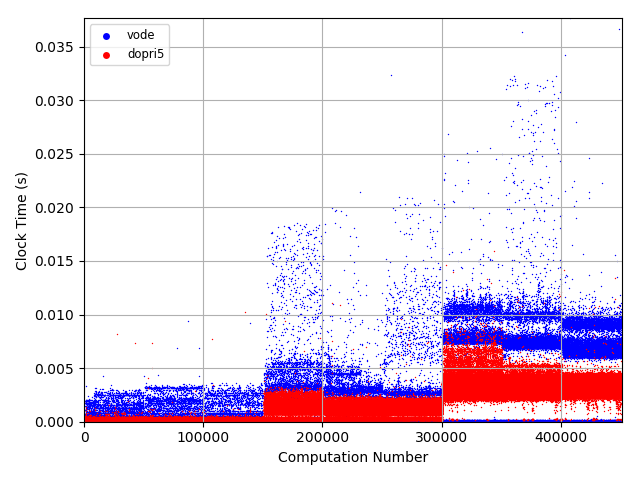
\includegraphics[width=\linewidth]{GRI_Mech_3/PaSR_Int_Times_1e-08.png}
%       \caption{Wall clock time required to integrate one time-step for both \texttt{dopri5} and \texttt{vode} at each particle of the PaSR model.}
%       \label{fig:WCTGRIPaSR}
%   \end{subfigure}
   \begin{subfigure}{0.43\textwidth}
       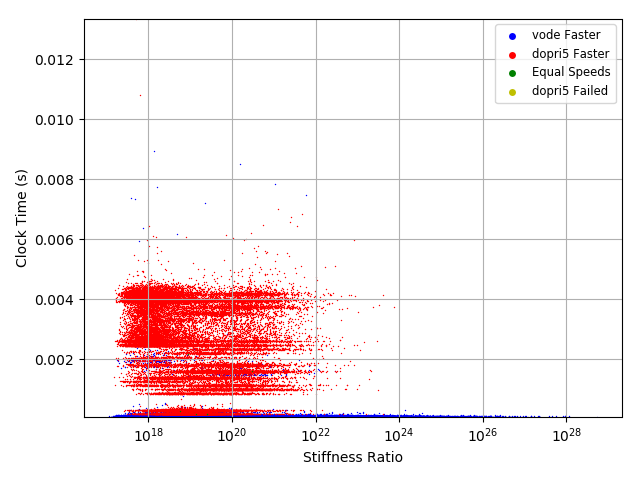
\includegraphics[width=\linewidth]{GRI_Mech_3/PaSR_Int_Times_Ratio_Groupings_1e-08.png}
       \caption{Stiffness ratio versus the wall clock time used to integrate one time-step at each particle of the PaSR model.}
       \label{fig:SRGRIPaSR}
   \end{subfigure}
    \hfill
   \begin{subfigure}{0.43\textwidth}
       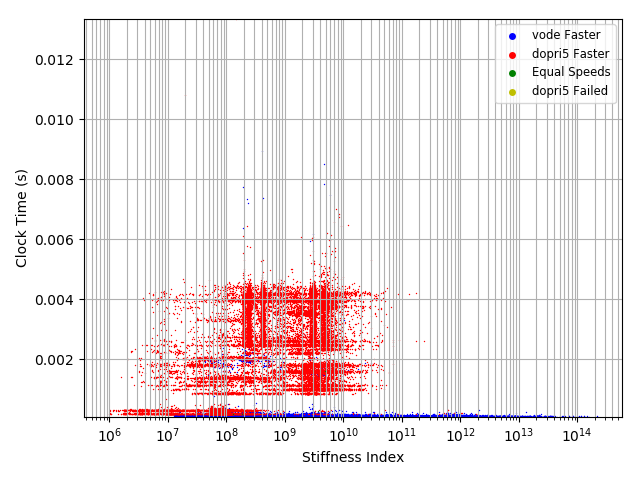
\includegraphics[width=\linewidth]{GRI_Mech_3/PaSR_Int_Times_Index_Groupings_1e-08.png}
       \caption{Stiffness index versus the wall clock time used to integrate one time-step at each particle of the PaSR model.}
       \label{fig:SI1GRIPaSR}
   \end{subfigure}
   \begin{subfigure}{0.43\textwidth}
       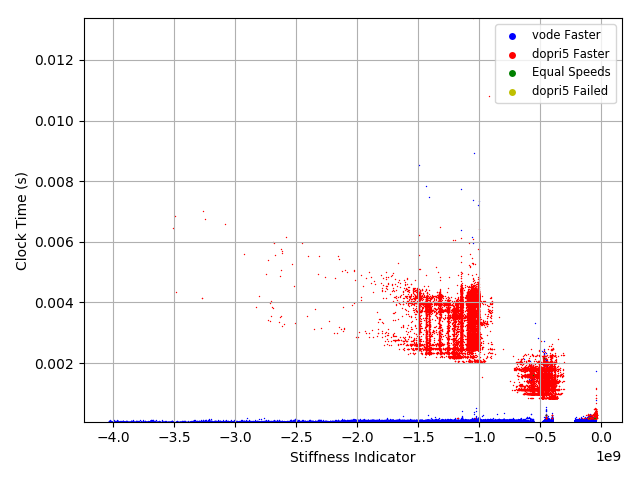
\includegraphics[width=\linewidth]{GRI_Mech_3/PaSR_Int_Times_Indicator_Groupings_1e-08.png}
       \caption{Stiffness indicator versus the wall clock time used to integrate one time-step at each particle of the PaSR model.}
       \label{fig:SI2GRIPaSR}
   \end{subfigure}
    \hfill   
   \begin{subfigure}{0.43\textwidth}
       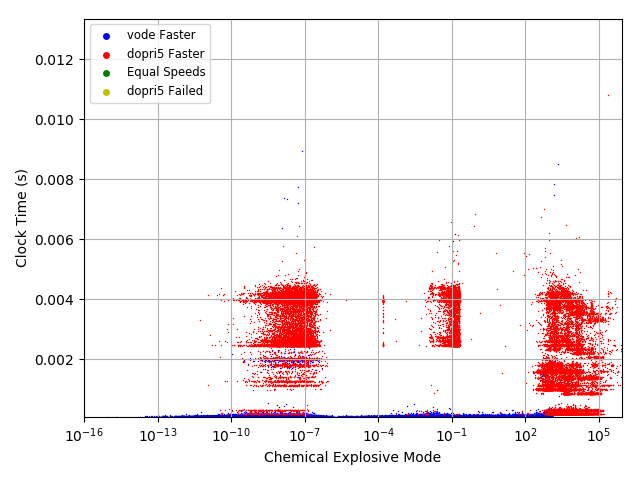
\includegraphics[width=\linewidth]{GRI_Mech_3/PaSR_Int_Times_CEMA_Groupings_1e-08.png}
       \caption{Chemical explosive mode versus the wall clock time used to integrate one time-step at each particle of the PaSR model.}
       \label{fig:CEMGRIPaSR}
   \end{subfigure}
   \caption{Stiffness metrics versus RHS function calls used to advance one time-step of the GRI Mech 3.0 model using either \texttt{vode} or \texttt{dopri5}.  Calculated with a constant step size of \SI{e-8}{\second} for every initial condition represented in the PaSR model.}
   \label{fig:GRIPaSRStiffness}
\end{figure}

As seen in Figure~\ref{fig:SRGRIPaSR}, the stiffness ratio was not correlated with the wall clock time required to integrate one time step, however \texttt{vode} appeared to generally outperform \texttt{dopri5} at values of the stiffness ratio greater than $10^{22}$.
At values of the stiffness ratio less than $10^{22}$, it is not clear which method has better performance.
The stiffness index behaved similarly to the stiffness ratio, as seen in Figure~\ref{fig:SI1GRIPaSR}
While the stiffness ratio was not correlated with the wall clock time required to integrate one time step, \texttt{vode} appeared to outperform \texttt{dopri5} at index values greater than approximately $5 \times 10^{10}$.

The usefulness of the stiffness indicator in predicting the wall clock time per time step was more clear in the set of data from the GRI Mech 3.0 model, as seen in Figure~\ref{fig:SI2GRIPaSR}.
Larger negative values of the stiffness indicator correspond to a longer wall clock time per integration for the \texttt{dopri5} integrator.
Further investigation will determine if additional trends may be made clear for the \texttt{vode} integrator if the time step were increased to a value larger than \SI{e-8}{\second}.
\texttt{vode} generally outperformed \texttt{dopri5} at values of the stiffness indicator value less than $-2 \times 10^{9}$ in the current set of data.
Additional investigation will determine if the stiffness indicator can reliably be used to predict relative performance of the two methods.

The usefulness chemical explosive mode in the GRI Mech 3.0 simulation was similar to the usefulness of the chemical explosive mode in the \ce{H2}\slash \ce{CO} simulation.
While the chemical explosive mode was not useful in predicting values of the wall clock time used to integrate one time step, \texttt{dopri5} outperformed \texttt{vode} when values of the chemical explosive mode were greater than $1.5 \times 10^2$.

We are interested in determining the potential speedup offered by an integrator using these metrics.
% May need a citation for this sentence.
Because implicit methods such as \texttt{vode} are used by default for most simulations of combustion, we are most interested in methods that predict when explicit methods such as \texttt{dopri5} have superior performance to explicit methods.
Using the data obtained from the simulations above, we are able to select integration times from either integrator based on stiffness metric values at those points.
For the set of data obtained from the GRI Mech 3.0 simulation, we selected the timing data from \texttt{vode} from particles that had a chemical explosive mode value of less than $1.5 \times 10^2$, and timing data from \texttt{dopri5} for all particles with a chemical explosive mode value of greater than $1.5 \times 10^2$.
The total clock time \texttt{vode} needed to integrate one time step at each particle of the PaSR simulation was 287.3 s, while the ``scheduler'' had a total wall clock time of 238.5 s to complete all integrations, a speedup of approximately 1.2$\times$ compared to \texttt{vode}.
For comparison, a perfect scheduler that selects the faster method at every particle would have a total integration time of 136.1 s, a speedup of approximately 2.1$\times$ compared to \texttt{vode}.

\section{Conclusions}
Four stiffness quantification metrics were investigated using partially stirred reactor simulations for two chemical kinetic models.
These metrics were the stiffness ratio, stiffness index, stiffness indicator, and the chemical explosive mode.
Our analysis demonstrated that the four stiffness quantification metrics investigated have the potential to be used by a scheduler that automatically selects the most efficient integration method at each point.
As an example, it was found that the wall clock time needed to integrate 450900 time steps of \SI{e-8}{\second} in the GRI Mech 3.0 model could have been reduced by a factor of 1.2$\times$ if a scheduler had selected an explicit method when the chemical explosive mode exceeded a value of $1.5 \times 10^2$.
Further analysis is needed to determine which stiffness quantification metric may be used to provide the largest speedup, as well as the sensitivity of these metrics to the user defined step size.
Additionally, the cost of determining the value of each stiffness quantification metric will be considered when implementing a scheduler in further research.

\section{Acknowledgements}
This material is based upon work supported by the National Science Foundation under grant ACI-1535065.

\setlength{\emergencystretch}{3em}
\printbibliography


\end{document}
